\documentclass[aspectratio=169,dvipdfmx,hyperref={bookmarks=true}]{beamer}
\usepackage{graphicx}
\usepackage{url}
\usepackage{bm}
\usepackage{amsmath}
\usepackage[absolute,overlay]{textpos}
\newcommand{\thickhrulefill}{\leavevmode\leaders\hrule depth-1.2pt height 3.2pt\hfill\kern0pt}
\newcommand{\indicatewidth}[1]{\thickhrulefill{#1}\thickhrulefill}
 \usetheme{Boadilla}
 \setbeamertemplate{navigation symbols}{}
 \setbeamertemplate{footline}[page number]
 \usepackage{algorithmic}
\usepackage{algorithm}
\usepackage{comment}
\usepackage{textcomp}
\usepackage{capt-of}
%\usepackage[dvipdfmx]{hyperref} % \movieref を使う場合に必要
\usepackage[dvipdfmx]{movie15_dvipdfmx}
%\usepackage[dvipdfmx]{movie15}
\usepackage {dotseqn}
\renewcommand{\kanjifamilydefault}{\gtdefault}% 既定をゴシック体に
\usepackage{caption}
\captionsetup[table]{labelformat=empty}
\captionsetup[figure]{labelformat=empty}

 %\usepackage[colorgrid,gridunit=pt,texcoord]{eso-pic}
 \title{煙シミュレーションのための部分空間法の高速化}
 \author{須之内 俊樹}
 \institute{中央大学理工学研究科 情報工学専攻 \\形状情報処理研究室 23N8100018B}
 \date{2025年 2月 21日}
 \usepackage{pxjahyper}
 \begin{document}
 %%%%%%%%%%%%%%%%%%%%%%%%%%%%%%%%%%%%%%%%%%%%%%%%%%%%%%%%%%%%%%%%%
   \begin{frame}
 \maketitle
 \end{frame} 
 %%%%%%%%%%%%%%%%%%%%%%%%%%%%%%%%%%%%%%%%%%%%%%%%%%%%%%%%%%%%%%%%%
% \begin{frame}
 %\tableofcontents
% \frametitle{目次}
 %\end{frame}
  %%%%%%%%%%%%%%%%%%%%%%%%%%%%%%%%%%%%%%%%%%%%%%%%%%%%%%%%%%%%%%%%%
  
  %1
     \section{概要}
 \begin{frame}
 \frametitle{概要}
 \begin{columns}[]
  %\vspace{-100pt}
 %\hspace{40pt}
	\begin{column}{0.3\linewidth}
	 \includemovie[autoplay, repeat,poster=movies/obstacle_origin.png,label=headorigin]{40mm}{40mm}{movies/obstacle_origin.mp4}
	 %	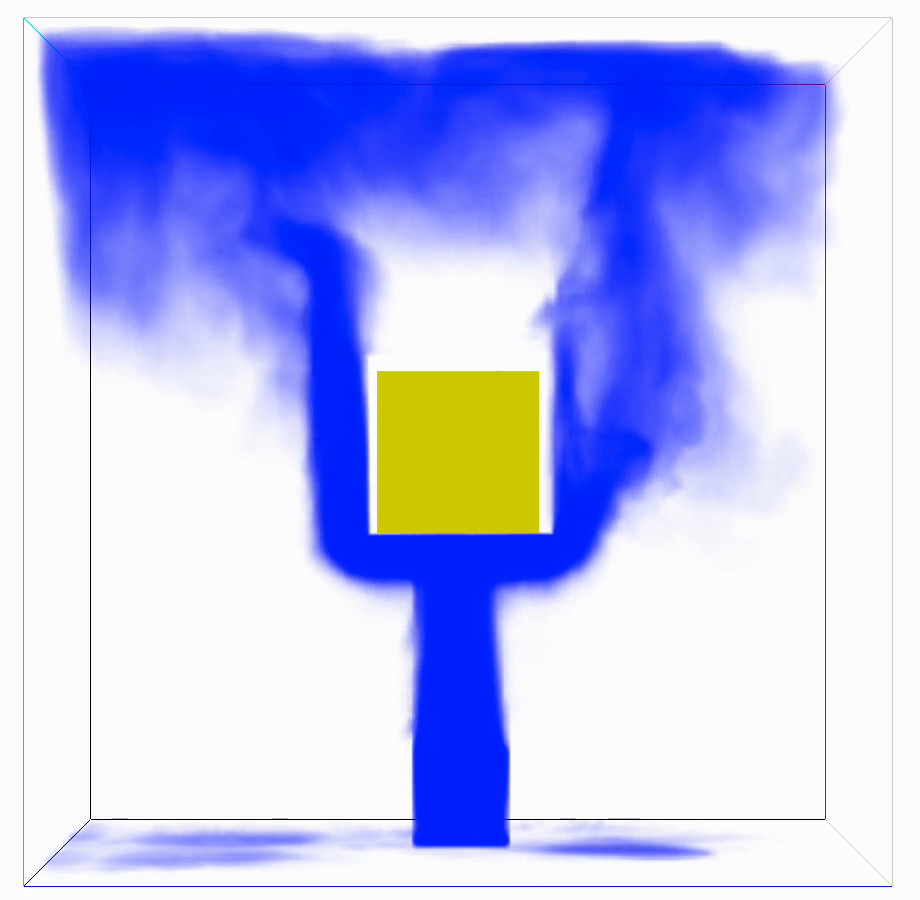
\includegraphics[width=1.0\linewidth]{movies/obstacle_origin.png}
	\end{column}
	\begin{column}{0.3\linewidth}
	\includemovie[autoplay, repeat,poster=movies/obstacle_dev2.png,label=headdev2]{40mm}{40mm}{movies/obstacle_dev4.mp4}
	%	 	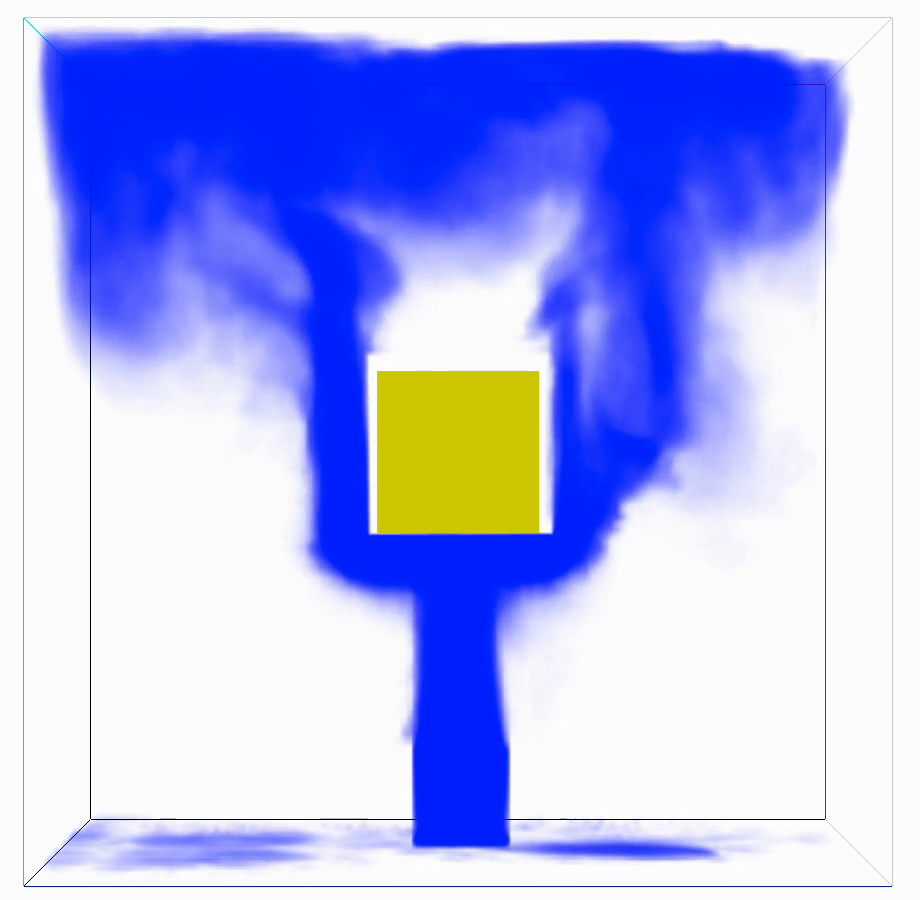
\includegraphics[width=1.0\linewidth]{movies/obstacle_dev4.png}
    \end{column}

	\begin{column}{0.35\linewidth}
	  \begin{block}{}
  		\begin{itemize}
			\item 190.54秒 $\to$ 33.43秒
		\end{itemize}
	\end{block}
    \end{column}
   \end{columns}

  \begin{block}{}
  \begin{itemize}
	\item 部分空間法:流体シミュレーションの高速化手法
	\item 煙のシミュレーションに部分空間法を適用
	\item 提案手法による部分空間法の高速化と,シミュレーション結果の変化を評価
\end{itemize}
\end{block}

 \end{frame}
%%%%%%%%%%%%%%%%%%%%%%%%%%%%%%%%%%%%%%%%%%%%%%%%%%%%%%%%%%%%%%%%%

%2
   \section{研究背景}
 \begin{frame}
 \frametitle{研究背景}
   \framesubtitle{流体シミュレーション}
 \subsection{流体シミュレーション}
%  \begin{block}{工業分野}
%  \begin{itemize}
%	\item 流体と接する製品の設計・製造
%	\item 物理的な正確さ
%\end{itemize}
%\end{block}
\begin{block}{CG分野}
\begin{itemize}
	\item 流体の映像の生成に利用
	\item 計算負荷の軽減,流体の挙動が制御しやすさ
	\item 物理的な正確さよりも,それらしさ
\end{itemize}
\end{block}

 \begin{block}{流体シミュレーションの課題}
  \begin{itemize}
\item 希薄な流体や,水飛沫は手法によっては再現できない
\item 近年は高品質な映像が求められ,計算負荷が大きい
%\item 部分空間法による計算負荷の削減に取り組む.
\end{itemize}
\end{block}
 \end{frame}
%%%%%%%%%%%%%%%%%%%%%%%%%%%%%%%%%%%%%%%%%%%%%%%%%%%%%%%%%%%%%%%%%
  %\begin{frame}
  %\frametitle{研究背景}
  %\framesubtitle{流体シミュレーションの数理モデル}
    %\begin{block}{ナビエ・ストークス方程式}
%\[
%\frac{\partial}{\partial t}\bm{u} = - (\bm{u} \boldsymbol{\cdot}\nabla) \bm{u} - \frac{1}{\rho}\nabla p + \nu\nabla^2\bm{u} + \bm{f}
%\]
%\[
%\nabla\boldsymbol{\cdot}\bm{u} = 0
%\]
%\begin{itemize}
%	\item $\bm{u}$,$\bm{f}$:流体の速度,外力
%	\item $p$,$\rho$,$\nu$:流体の圧力,密度,粘性
%	\item $\nabla = ( \frac{\partial}{\partial x}, \frac{\partial}{\partial y}, \frac{\partial}{\partial z})$
%\end{itemize}
%\end{block}
%\end{frame}
%%%%%%%%%%%%%%%%%%%%%%%%%%%%%%%%%%%%%%%%%%%%%%%%%%%%%%%%%%%%%%%%%

%3
  \begin{frame}
  \frametitle{研究背景}
  \framesubtitle{流体シミュレーション(煙,液体)の数理モデル}

\begin{columns}[T]
	\begin{column}{0.65\linewidth}
	    \begin{block}{ナビエ・ストークス方程式の離散化}
    	\[
	\bm{u}(t + \varDelta t)  =\bm{u}(t) -\varDelta t( (\bm{u} \boldsymbol{\cdot}\nabla) \bm{u} - \frac{1}{\rho}\nabla p + \nu\nabla^2\bm{u} + \bm{f})
	\]
	\[
	\nabla\boldsymbol{\cdot}\bm{u} = 0
	\]
	\vspace{-10pt}
	\begin{itemize}
	\item $\bm{u}$,$\bm{f}$:流体の速度,外力
	\item $p$,$\rho$,$\nu$:流体の圧力,密度,粘性
	\item $\nabla = ( \frac{\partial}{\partial x}, \frac{\partial}{\partial y}, \frac{\partial}{\partial z})$
\end{itemize}
\end{block}
	\begin{block}{スタッガード格子}
		\begin{itemize}
		\item 速度と圧力の配置位置を工夫し,計算の安定性を向上
		\item 非直交格子への適用が困難
	\end{itemize}
	\end{block}
    	\end{column}
	\begin{column}{0.35\linewidth}
	%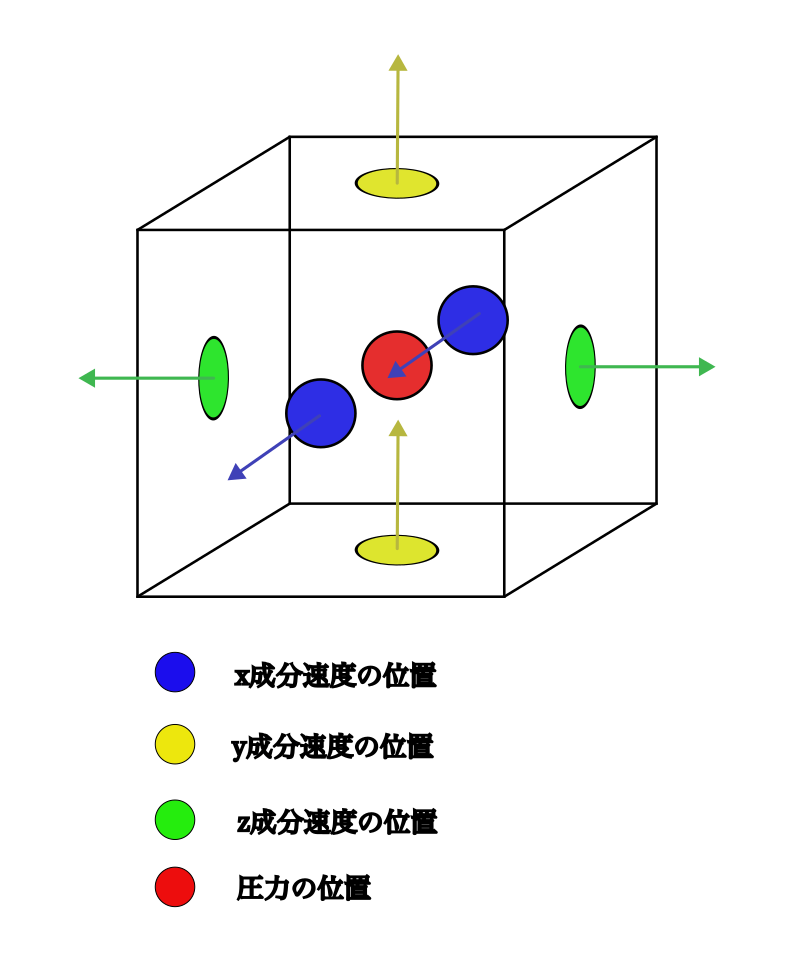
\includegraphics[width=1.1\linewidth]{images/3dstaggerd.png}
	%\vspace{-10pt}
	\includegraphics[width=0.9\linewidth]{images/Macgrid.png}
	\label{fig:staggerd}
    	\end{column}
    \end{columns}
\end{frame}
%%%%%%%%%%%%%%%%%%%%%%%%%%%%%%%%%%%%%%%%%%%%%%%%%%%%%%%%%%%%%%%%%

%4
  \begin{frame}
  \frametitle{研究背景}
  \framesubtitle{流体シミュレーション(煙,液体)の数理モデル}
    \begin{block}{部分段階法}
    	\[
	\bm{u}(t + \varDelta t)  =\bm{u}(t) -\varDelta t( (\bm{u} \boldsymbol{\cdot}\nabla) \bm{u} - \frac{1}{\rho}\nabla p + \nu\nabla^2\bm{u} + \bm{f})
	\]
中間子$\bm{u}_0$から$\bm{u}_3$を用いて,以下のように各項ごとに分割して計算する

\begin{align*}
	\bm{u}_0				& =  \bm{u} (t)  - \varDelta t \bm{f} 				\\
	\bm{u}_1 (\bm{x}) 		&= \bm{u}_0 (\bm{x}) - \varDelta t (\bm{u}_0(\bm{x})  \boldsymbol{\cdot}\nabla) \bm{u}_0(\bm{x})	\\
	\bm{u}_2  		 		&=  \bm{u}_1 - \varDelta t \nu\nabla^2\bm{u}_1		\\
	\bm{u} (t + \varDelta t) = \bm{u}_3  &=  \bm{u}_2 - \varDelta t \frac{1}{\rho}\nabla \bm{p}
\end{align*}
%\[
%	\bm{u}_0 =  \bm{u} (t)  - \varDelta t \bm{f} 
%\]
%\[
%	\bm{u}_1 (\bm{x}) = \bm{u}_0 (\bm{x}) - \varDelta t (\bm{u}_0(\bm{x})  \boldsymbol{\cdot}\nabla) \bm{u}_0(\bm{x})
	%\bm{u}_1(\bm{x}) = \bm{u}_0(\bm{x}  - \varDelta t \bm{u}_0)
%\]
%\[
%	\bm{u}_2   =  \bm{u}_1 - \varDelta t \nu\nabla^2\bm{u}_1
%\]
%\[
%	\bm{u} (t + \varDelta t) = \bm{u}_3  =  \bm{u}_2 - \varDelta t \frac{1}{\rho}\nabla \bm{p} 
%\]
\end{block}
\end{frame}
%%%%%%%%%%%%%%%%%%%%%%%%%%%%%%%%%%%%%%%%%%%%%%%%%%%%%%%%%%%%%%%%%

%5
  \begin{frame}
  \frametitle{研究背景}
  \framesubtitle{流体シミュレーション(煙,液体)の数理モデル}
    \begin{block}{部分段階法}
%\begin{align}
\begin{eqnarray}
%\begin{array}{ccc}
	\bm{u}_0			&=&  \bm{u} (t)  - \varDelta t \bm{f}\notag \\ 
	\bm{u}_1(\bm{x}) 	&=& \bm{u}_0(\bm{x}  - \varDelta t \bm{u}_0)\label{eq:semi-Lagrangian}\\
	\bm{u}_2   		&=&  \bm{V}\bm{u}_1		\notag\\
	\bm{b} 			&=& \bm{W}\bm{u}_2		 \label{eq:v2p}	\\ 
	\bm{p} 			&=& \bm{A}^{-1}\bm{b}	\label{eq:poisson} \\ 
	\bm{u} (t + \varDelta t) = \bm{u}_3  	&=& \bm{u}_2 - \bm{Y}\bm{p}\notag
%\end{array}
%\end{align}
\end{eqnarray}

\begin{itemize}
\item 式\ref{eq:semi-Lagrangian}はsemi-Lagrangian法[Stam 1999],式\ref{eq:v2p},\ref{eq:poisson}はコリンの射影法[Chorin 1968]
\item $\bm{V}$,$\bm{A}$は離散ラプラシアン行列を用いて$\nabla^2$を離散化
\item $\bm{W}$,$\bm{Y}$は勾配演算子$\nabla$を離散化
\end{itemize}
\end{block}
\end{frame}
%%%%%%%%%%%%%%%%%%%%%%%%%%%%%%%%%%%%%%%%%%%%%%%%%%%%%%%%%%%%%%%%%
%6

\begin{frame}
 \frametitle{研究背景}
   \framesubtitle{先行研究}
\begin{columns}[T]
	\begin{column}{0.6\linewidth}
	\begin{block}{Visual Simulaton of Smoke [Fedkiw et al. 2001]}
		\begin{itemize}
		\item CGにおいて広く用いられる煙のオフラインシミュレーション手法
		\item 密度を計算した後,ボリュームレンダリングを用いて描画
		\item 計算量は空間解像度に依存
	\end{itemize}
	\end{block}
	
	\begin{block}{計算機実験}
	\begin{itemize}
	\item 解像度$128^3$,$200$フレーム
	\item シミュレーション\text{1800ms/f}
	\item レンダリング\text{240ms/f}
	\end{itemize}
	\end{block}
    	\end{column}
	\begin{column}{0.4\linewidth}
\includemovie[autoplay, repeat,poster=movies/obstacle_origin.png, label=hikone]{60mm}{60mm}{movies/obstacle_origin.mp4}
%		 	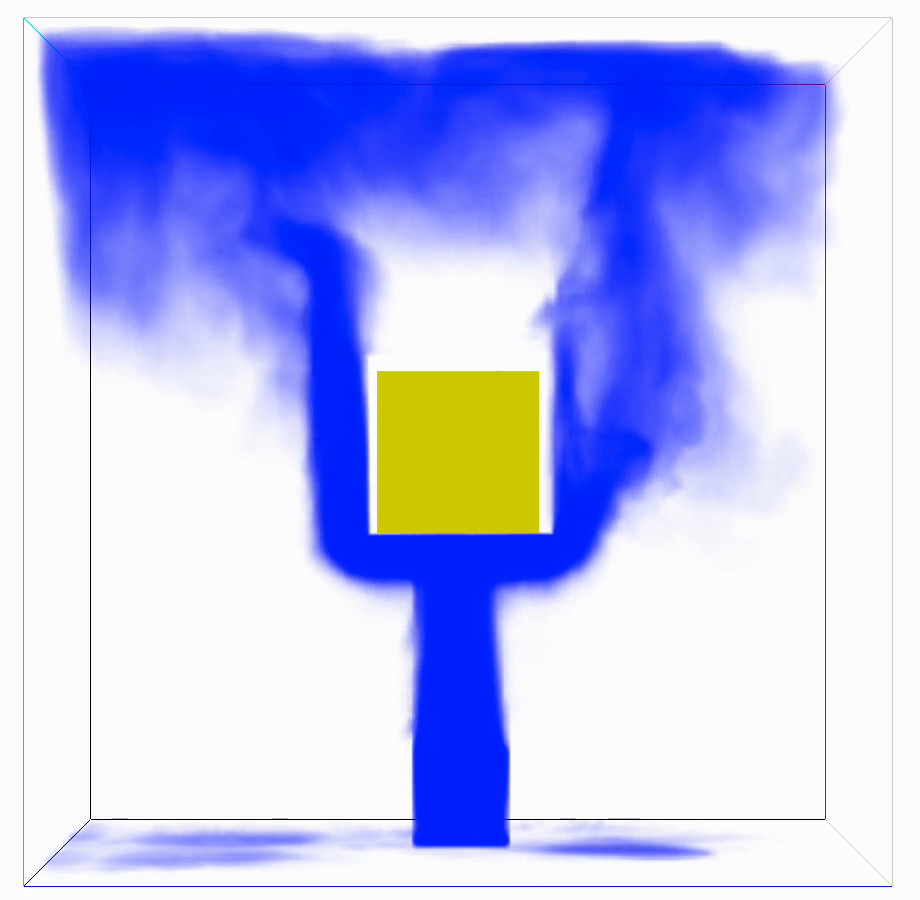
\includegraphics[width=1.0\linewidth]{movies/obstacle_origin.png}
    	\end{column}
    \end{columns}
 \end{frame}
  %%%%%%%%%%%%%%%%%%%%%%%%%%%%%%%%%%%%%%%%%%%%%%%%%%%%%%%%%%%%%%%%%
  
  %7
  \begin{comment}
\begin{frame}
 \frametitle{研究背景}
    \framesubtitle{煙シミュレーションの先行研究}
   \begin{block}{ボリュームレンダリング}
   \begin{itemize}
 	\item 3次元空間の全てのボクセル値を可視化画像に反映させるレンダリング手法
	\item 透明度を考慮したレンダリングに用いられる
\end{itemize}
\end{block}
\begin{columns}[T]
	\begin{column}{0.6\linewidth}
	\begin{algorithm}[H]
    		\caption{Axis Alined slice-based Volume Rendering}
       	 \label{alg1}
        		\begin{algorithmic}[1]
                        \STATE x,y,z軸の中から,視線方向に近いものを選ぶ
                        \STATE 軸に垂直な平面(スライス)を,アルファブレンディングして描画
                        \[{\rm{I}}_n= \alpha_n c_n + (1-\alpha_n){\rm{I}}_{n-1}\]
                        \[\alpha= 1 - \exp(-\rho\Delta s)\]
            	\end{algorithmic}
	\end{algorithm}
    	\end{column}
	
	\begin{column}{0.4\linewidth}
	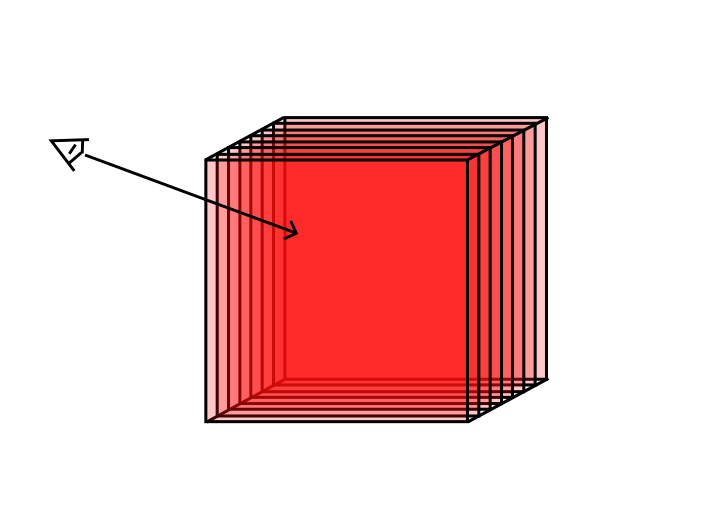
\includegraphics[width=\linewidth]{images/slice_base.png}
    	\end{column}
    \end{columns}
 \end{frame}
\end{comment}
  %%%%%%%%%%%%%%%%%%%%%%%%%%%%%%%%%%%%%%%%%%%%%%%%%%%%%%%%%%%%%%%%%
  
  %8
   \begin{frame}
  \frametitle{研究背景}
      \framesubtitle{部分空間法}
\begin{block}{部分空間法(subspace method)}
\begin{itemize}
\item 既存のシミュレーションの時系列データ(スナップショット)を主成分分析し,次元削減する
%\end{itemize}
%\end{block}
%\begin{block}{概要}
%\begin{itemize}
% \item シミュレーションの前処理として,$\bm{A}^{\mathsf T} \bm{A} = \bm{I}$を満たし,$\bm{x} = \bm{A}\bm{\widetilde{x}} $が成り立つような,$n \times r$行列$\bm{A}$を考える
 %\[
 %\bm{\widetilde{x}} = \bm{A}^{\mathsf T}\bm{x}
 %\]
%\item $\bm{\widetilde{x}}$を用いてシミュレーションを行い,$\bm{x} = \bm{A}\bm{\widetilde{x}}$を用いて$\bm{x}$を求める
\item 本研究の高速化の対象は,主成分分析
\end{itemize}
\end{block}
\begin{block}{流体シミュレーションへの適用}
\begin{itemize}
	\item 空間解像度を保ったまま高速化可能
	\item タイムステップを小さくして再計算できる
	\item 前処理の計算負荷が大きい
	\item 次元削減後の流速$\bm{\widetilde{u}}$は,流体の非圧縮条件$\nabla\boldsymbol{\cdot}\bm{\widetilde{u}}$ = 0を満たしていなければならない
\end{itemize}
\end{block}
%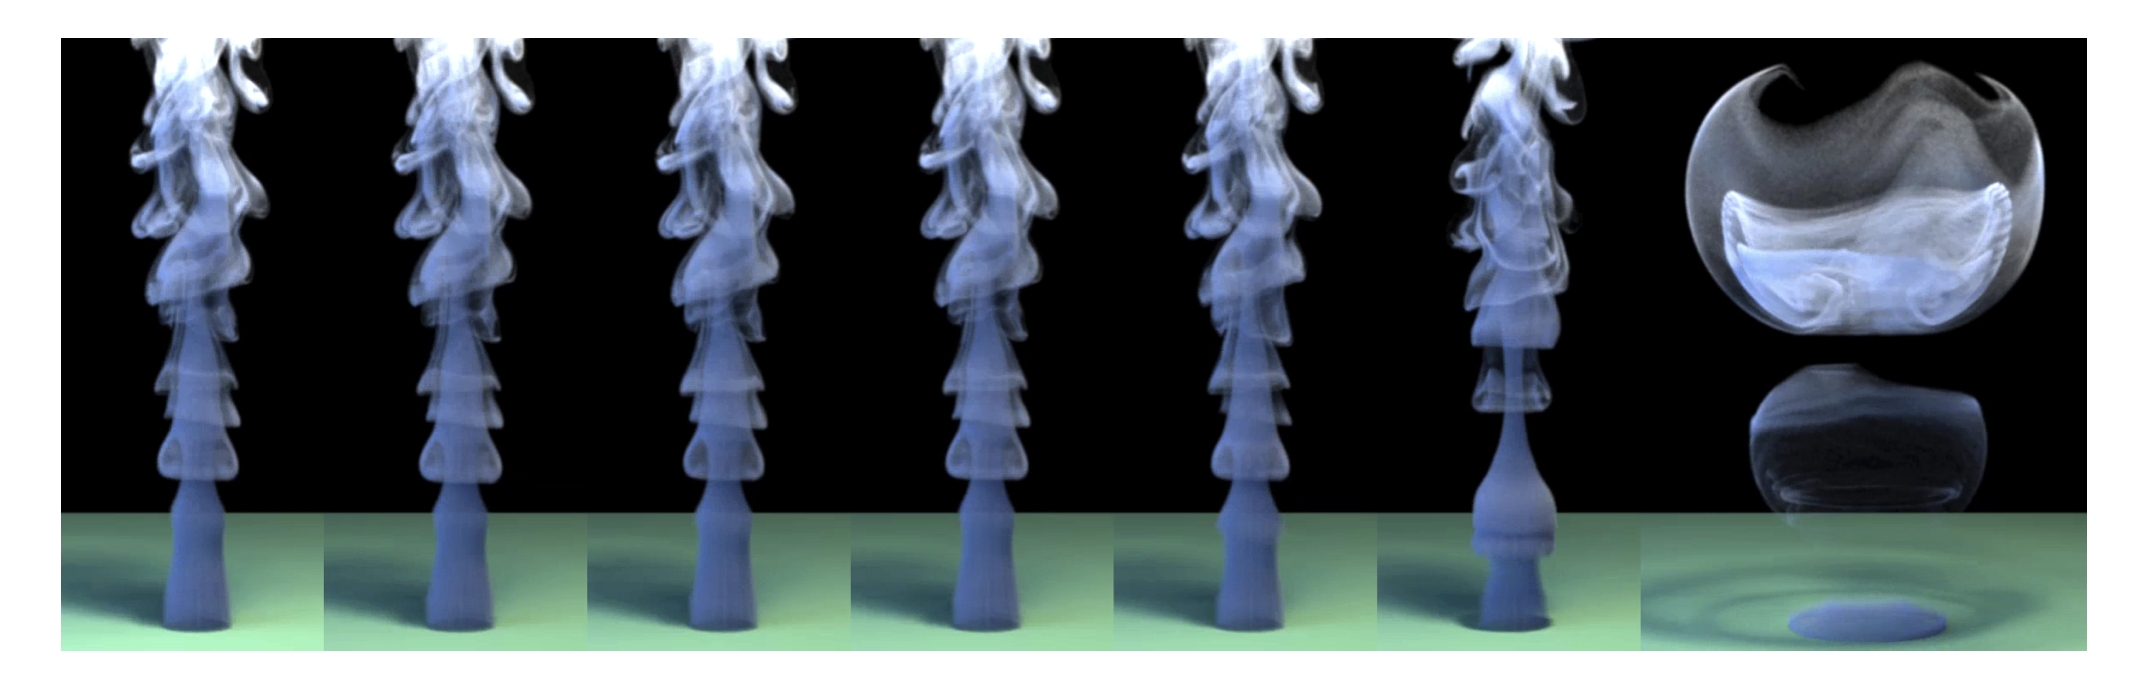
\includegraphics[width=0.7\linewidth]{images/subspace.png}
 \end{frame}
%%%%%%%%%%%%%%%%%%%%%%%%%%%%%%%%%%%%%%%%%%%%%%%%%%%%%%%%%%%%%%%%%

%9
   \begin{frame}
  \frametitle{研究背景}
    \framesubtitle{部分空間法}
   \begin{block}{特異値分解を用いた直交基底の計算}
   \begin{itemize}
   \item 既存のシミュレーションの時系列データ(スナップショット)を$T$個用いて,部分空間の直交基底を作成する手法
\item 空間解像度を$n$,削減後の次元を$r$とすると,$n <\!< T <\!< r$ 
\item 時刻$t$における速度ベクトル$\bm{u_t}$を用いて,$3(n+1)\times T$行列$\bm{S}$を定義する
	 \[ \bm{S} = 
        		\begin{bmatrix}
   \bm{u}_0 & \bm{u}_1 &\cdots  & \bm{u}_{T-1}
\end{bmatrix}
\]
\item $\bm{S}$を特異値分解して得られる左特異行列$\bm{U}$を部分空間の直交基底とする
\item 先にQR分解を適用し,サイズを小さくすることができる
\end{itemize}
\end{block}

%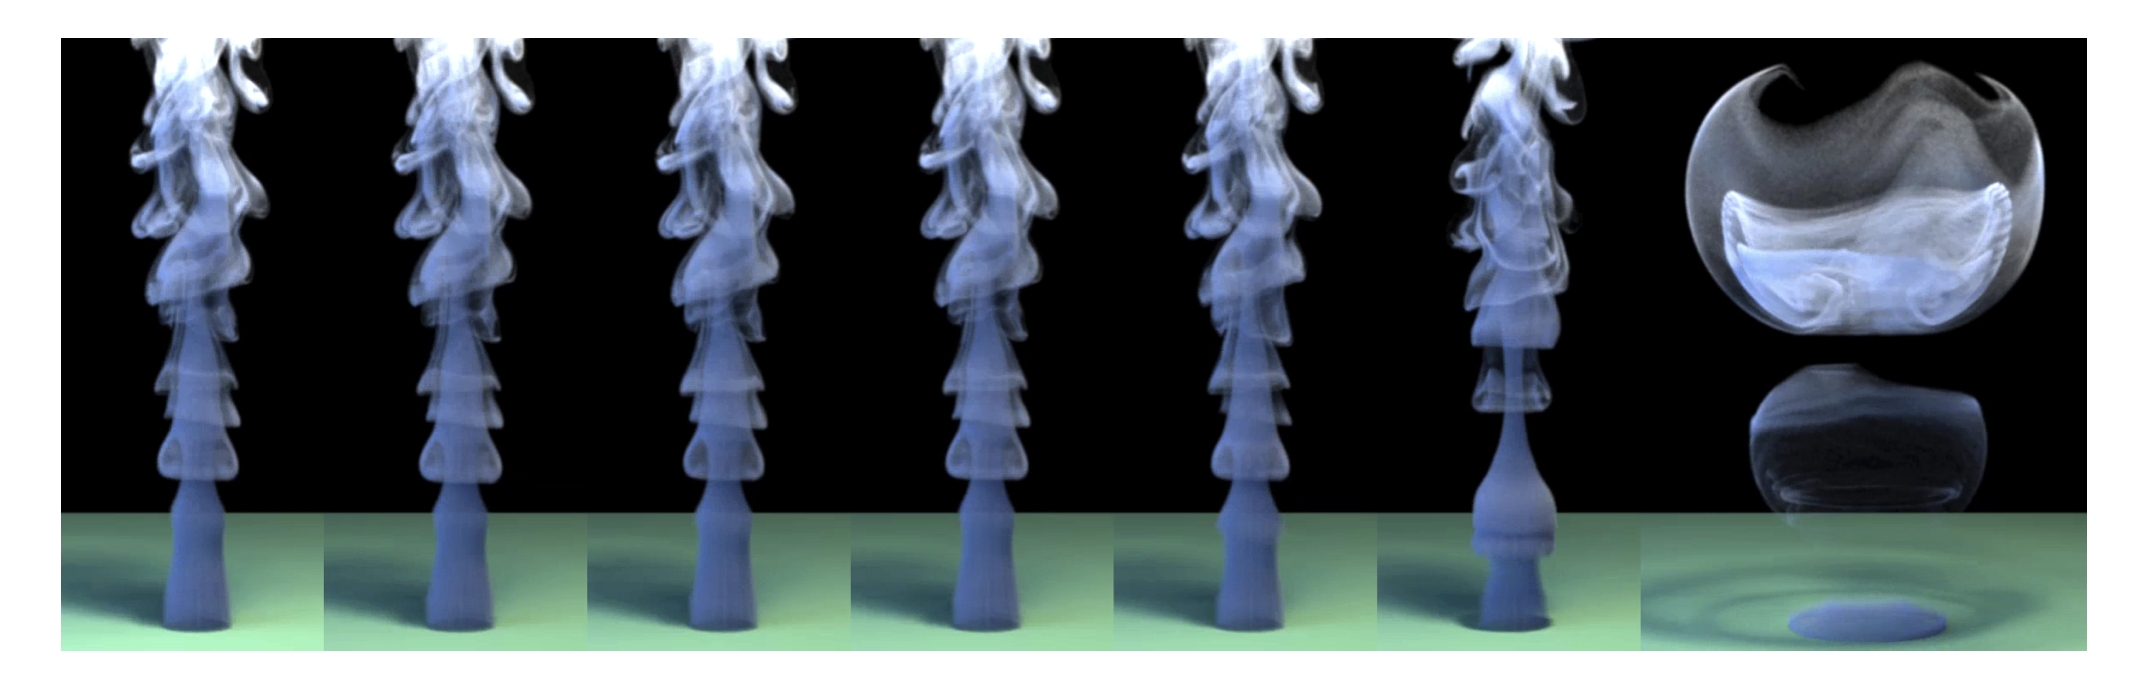
\includegraphics[width=0.7\linewidth]{images/subspace.png}
 \end{frame}
 %%%%%%%%%%%%%%%%%%%%%%%%%%%%%%%%%%%%%%%%%%%%%%%%%%%%%%%%%%%%%%%%%
 
 %10
\begin{frame}
\frametitle{研究背景}
\framesubtitle{先行研究}
	\begin{block}{部分空間上のシミュレーション手法[Treuille et al. 2006]}
	   \begin{itemize}
   	\item 中間子$\bm{u}_i$から得た基底を$\bm{U}_i$,$\bm{p}$から得られた基底を$\bm{P}$とする
	\item $n\times n$行列が$r \times r$行列に.各ステップが高速化
	\item 前処理に$\bm{\widetilde{V}}$,$\bm{\widetilde{W}}$,$\bm{\widetilde{A}}$,$\bm{\widetilde{Y}}$の計算も含める
	\end{itemize}
\begin{align*}
 \bm{u}_2   		&=  \bm{V}\bm{u}_1&\bm{U}_2^{\mathsf T}\bm{u}_2	& = (\bm{U}_2^{\mathsf T}\bm{V}\bm{U}_1)\bm{U}_1^{\mathsf T}\bm{u}_1 					&\bm{\widetilde{u}}_2 		&= \bm{\widetilde{V}}\bm{\widetilde{u}_1}	\\
 \bm{b} 			&= \bm{W}\bm{u}_2&\bm{P}^{\mathsf T}\bm{b}		& = (\bm{P}^{\mathsf T}\bm{W}\bm{U}_2)\bm{U}_2^{\mathsf T}\bm{u}_2        				&\bm{\widetilde{b}}			&= \bm{\widetilde{W}}\bm{\widetilde{u}}_2	\\
 \bm{p} 			&= \bm{A}^{-1}\bm{b}&\bm{P}^{\mathsf T}\bm{p} 		&= (\bm{P}^{\mathsf T}\bm{A}^{-1}\bm{P})\bm{P}^{\mathsf T}\bm{b}						&\bm{\widetilde{p}}			&= \bm{\widetilde{A}}\bm{\widetilde{b}}\\
\bm{u}_3  			&= \bm{u}_2 - \bm{Y}\bm{p} &\bm{U}_3^{\mathsf T}\bm{u}_3 	&=  \bm{U}_2^{\mathsf T}\bm{u}_2 - (\bm{U}_3^{\mathsf T}\bm{Y}\bm{P})\bm{P}^{\mathsf T}\bm{p}	&\bm{\widetilde{u}}_3		&= \bm{\widetilde{u}}_2  -  \bm{\widetilde{Y}}\bm{\widetilde{p}}
\end{align*}
\end{block}
%	\begin{block}{非線形項}
 %		\begin{itemize}
%		\item 立体求積法\cite{subspace}[Kim et al.2013]を用いる
%		\item 本研究の高速化の対象ではない
%	\end{itemize}
%	\end{block}
\end{frame}
%%%%%%%%%%%%%%%%%%%%%%%%%%%%%%%%%%%%%%%%%%%%%%%%%%%%%%%%%%%%%%%%%

%\begin{frame}
%\frametitle{研究背景}
%\framesubtitle{先行研究}
%	\begin{block}{非線形項}
% 		\begin{itemize}
%		\item 立体求積法\cite{subspace}[Kim et al.2013]を用いる.
%		非線形関数$\mathcal{F}$について,$\bm{f} = \mathcal{F}(\bm{x})$とする.
%\[
%	\bm{f} = \int_\Omega\mathcal{F}_p(\bm{x}_p) = \sum_{p=1}^Pw_p\mathcal{F}_p(\bm{x}_p)
%\]
%\item $\Omega$:シミュレーション領域.
%\item $P$:サンプリングした点集合,
%\item $w_p$:サンプリング点$p$に対応する重み
%		\end{itemize}
%	\end{block}
%\end{frame}

%%%%%%%%%%%%%%%%%%%%%%%%%%%%%%%%%%%%%%%%%%%%%%%%%%%%%%%%%%%%%%%%%

%\begin{frame}
%\frametitle{研究背景}
%\framesubtitle{先行研究}
%	\begin{block}{非線形項}
 %		\begin{itemize}
%		\item 速度に関する基底を用いて部分空間へ射影する.
%\[
%	\bm{U}_1\bm{f} = \sum_{p=1}^Pw_p(\bm{U}^p)^{\mathsf T}\mathcal{F}_p(\bm{U}^p\bm{x})
%\]
%\item $\bm{U}^p$:$\bm{U}$から$p$に関する行を抜粋した$3 \times n$行列
%$\bm{\widetilde{f}}_p$ = $(\bm{U}^p)^{\mathsf T}\mathcal{F}_p(\bm{\widetilde{u}})$とする
%		\end{itemize}
%	\end{block}
%\end{frame}
%%%%%%%%%%%%%%%%%%%%%%%%%%%%%%%%%%%%%%%%%%%%%%%%%%%%%%%%%%%%%%%%%

%11
\begin{frame}
\frametitle{部分空間法の課題}
\subsection{部分空間法の課題}
	\begin{block}{空間計算量}
		一般に,
		\[64^3 \le n \le 1024^3\]
		\[30 \le r \le 150\]
   		\begin{itemize}
			\item $n = 256^3$,$r=50$のとき,行列$\bm{A}$のために10GBほど必要
			\item 廉価なGPUではメモリが足りない
   			\item 削減後の次元の数に制限.$r \le T$
		\end{itemize}
	\end{block}

	\begin{block}{前処理の計算時間}
 		\begin{itemize}
		\item $3(n +1)\times T$行列の特異値分解,QR分解の計算量は$O(nT^2)$
		\item	シミュレーションに用いる行列を,部分空間へ射影する計算時間
		%\item 非線形項:$O(rTP^3)$
	\end{itemize}
	\end{block}
\end{frame}
%%%%%%%%%%%%%%%%%%%%%%%%%%%%%%%%%%%%%%%%%%%%%%%%%%%%%%%%%%%%%%%%%

%12
\section{提案手法}
\begin{frame}
\frametitle{提案手法}
\begin{block}{スナップショットの分割}
 \[ \bm{S} = 
        		\begin{bmatrix}
   \bm{u}_0 & \bm{u}_1 &\cdots  & \bm{u}_{T-1}
\end{bmatrix}
\]
二分割すると,
%\begin{align*}
\begin{eqnarray}
	\bm{S_0} 		&= \begin{bmatrix}\bm{u}_0 &\cdots  & \bm{u}_{T/2-1}\end{bmatrix}\notag		\\
	\bm{S_1} 	&= \begin{bmatrix} \bm{u}_{T/2}  &\cdots  & \bm{u}_{T-1}\end{bmatrix}\notag	
\end{eqnarray}
%\end{align*}
$O(nT^2)$の計算負荷が,$O(2n(T/4))$に削減できる
\end{block}

\begin{block}{評価方法}
 	\begin{itemize}
	\item 前処理の計算時間を計測
	\item	累積寄与率を計測
	\item	相対誤差により精度を評価
	%\item 非線形項:$O(rTP^3)$
	\end{itemize}
\end{block}


 \end{frame}

  %%%%%%%%%%%%%%%%%%%%%%%%%%%%%%%%%%%%%%%%%%%%%%%%%%%%%%%%%%%%%%%%%
  
  %13
 \begin{frame}
 \frametitle{実験結果}
 \vspace{-25pt}
 \begin {table}[htbp]
    \centering
  \caption{基底計算の解像度と分割数ごとの実行時間(秒)}
  \label{tab:basis}
  \begin {tabular}{rrrrr} \hline
    \multicolumn{1}{c}{解像度} 					&\multicolumn{1}{c}{分割なし} 		&\multicolumn{1}{c}{分割数2}			&\multicolumn{1}{c}{分割数4} 		&\multicolumn{1}{c}{分割数10}\\ \hline
    $64^3$ 					& 23.43 			&14.56	 		&8.98	 	&3.78\\
    $128^3$ 				& 190.54 			&118.49 			& 69.62 		&33.43\\ \hline
  \end {tabular}
\end {table}

\begin {table}[htbp]
    \centering
  \caption{行列の射影の解像度と分割数ごとの実行時間(秒)}
  \label{tab:projection}
  \begin {tabular}{rrrrr} \hline
    \multicolumn{1}{c}{解像度} 					&\multicolumn{1}{c}{分割なし} 		&\multicolumn{1}{c}{分割数2}			&\multicolumn{1}{c}{分割数4} 		&\multicolumn{1}{c}{分割数10}\\ \hline
    $64^3$ 					& 3.51 			&2.82	 		&0.85	 		&0.67\\
    $128^3$ 				& 5.21 			& 3.06 			& 3.05 			&3.98\\ \hline
  \end {tabular}
\end {table}

\begin {table}[htbp]
    \centering
  \caption{基底の累積寄与率の最小値(上)と最大値(下)}
  \label{tab:ruiseki}
  \begin {tabular}{rrrrr} \hline
    \multicolumn{1}{c}{解像度} 					&\multicolumn{1}{c}{分割なし} 		&\multicolumn{1}{c}{分割数2}			&\multicolumn{1}{c}{分割数4} 		&\multicolumn{1}{c}{分割数10}\\ \hline
    $64^3$ 									& 0.970						& 0.972							&0.98		 				&0.993				\\
    										&							&0.986							&0.990						&0.997				\\ \hline
    $128^3$ 								&0.940 						&0.955							&0.971		 				&0.989				\\ 
    										&							&0.965							&0.976						&0.996				\\	\hline
  \end {tabular}
\end {table}
\end{frame}
%%%%%%%%%%%%%%%%%%%%%%%%%%%%%%%%%%%%%%%%%%%%%%%%%%%%%%%%%%%%%%%%%

%14
\section{提案手法}
\begin{frame}
\frametitle{実験結果}
	%\begin{column}{0.3\linewidth}
%	\begin{block}{}
%	平均誤差$L_2 = \frac{|| \bm{u} - \bm{\widetilde{u}} ||_2}{||  \bm{u} ||_2}$
%	\end{block}
	%\end{column}
%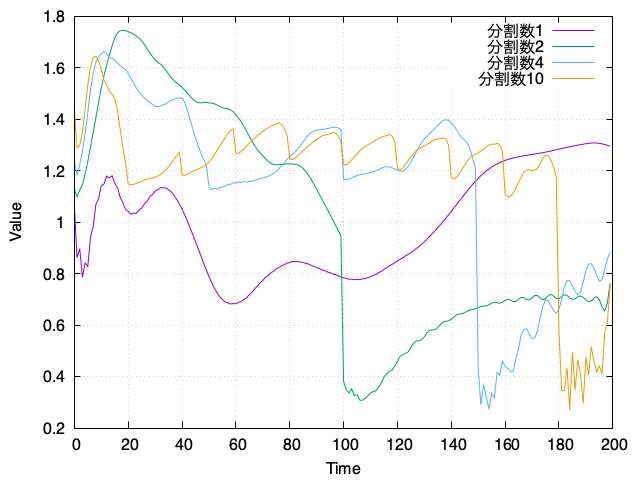
\includegraphics[width=0.8\linewidth]{images/128error.png}
\vspace{-10pt}
\begin{columns}[T]
	\begin{column}{0.15\linewidth}
	\begin{block}{}
	相対誤差$L_2 = \frac{|| \bm{u} - \bm{\widetilde{u}} ||_2}{||  \bm{u} ||_2}$
	\end{block}
    	\end{column}
	\begin{column}{0.85\linewidth}
	\vspace{-20pt}
		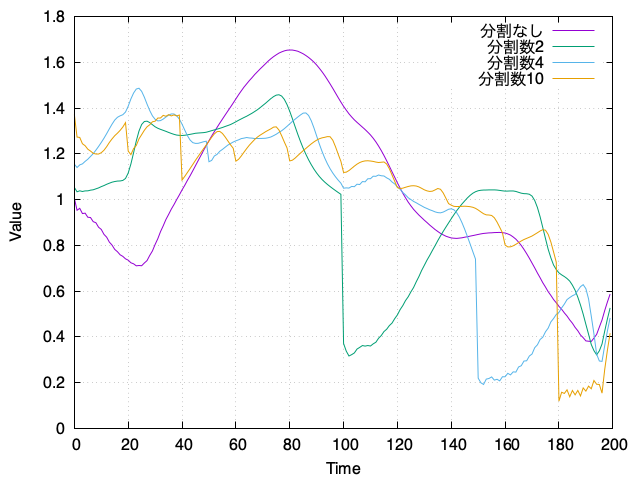
\includegraphics[width=0.9\linewidth]{images/128error_obstacle.png}
	   \end{column}
    \end{columns}
 \end{frame}
  %%%%%%%%%%%%%%%%%%%%%%%%%%%%%%%%%%%%%%%%%%%%%%%%%%%%%%%%%%%%%%%%%
  
  %15
 \begin{frame}
 \frametitle{実験結果}
%sub diff 6micro
%sub proj 4micro
%sub restore 1800micro
\begin{block}{}
解像度$128^3$,$200$フレーム

CPU:Apple M4 Pro,メモリ:64GB

分割前後で流れが変化しているのが確認できる.
\end{block}
\begin{columns}
    \begin{column}{0.33\textwidth}
   \begin{figure}
\includemovie[autoplay, repeat,poster=movies/obstacle_origin.png, label=origin]{40mm}{40mm}{movies/obstacle_origin.mp4}
%		 	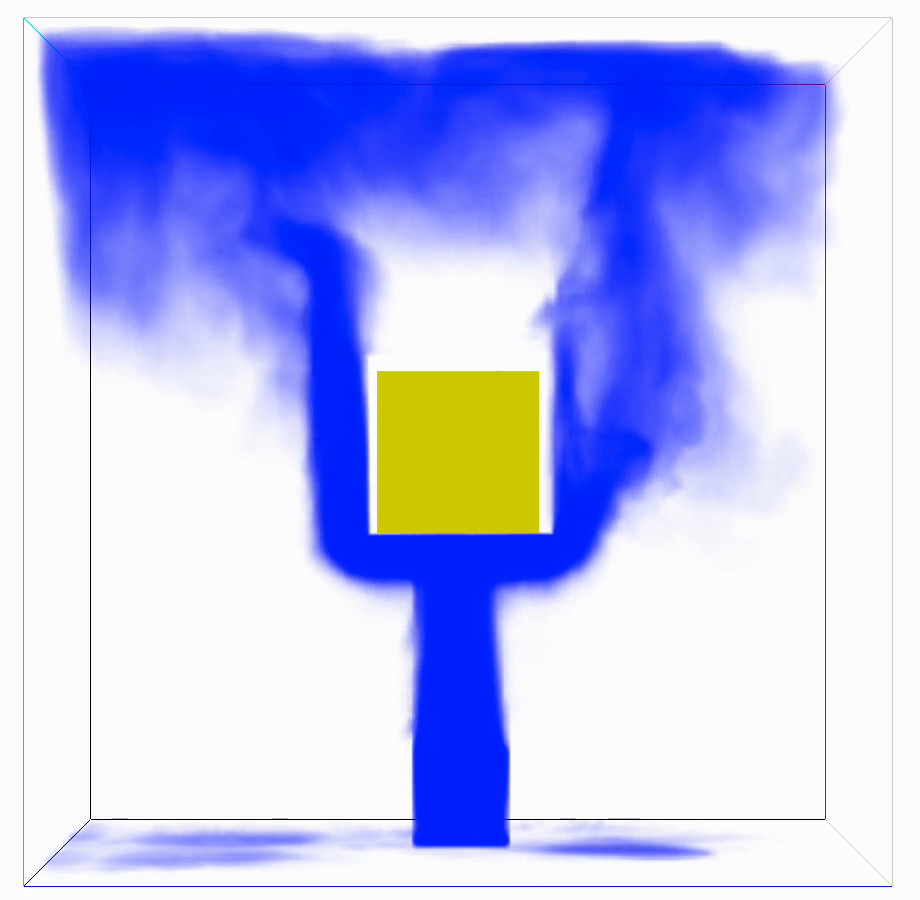
\includegraphics[width=1.0\linewidth]{movies/obstacle_origin.png}
\caption{オリジナルのシミュレーション}
   \end{figure}
    \end{column}
    \begin{column}{0.33\textwidth}
       \begin{figure}
\includemovie[autoplay, repeat,poster=movies/obstacle_dev1.png, label=dev1]{40mm}{40mm}{movies/obstacle_dev1_color.mp4}
%		 	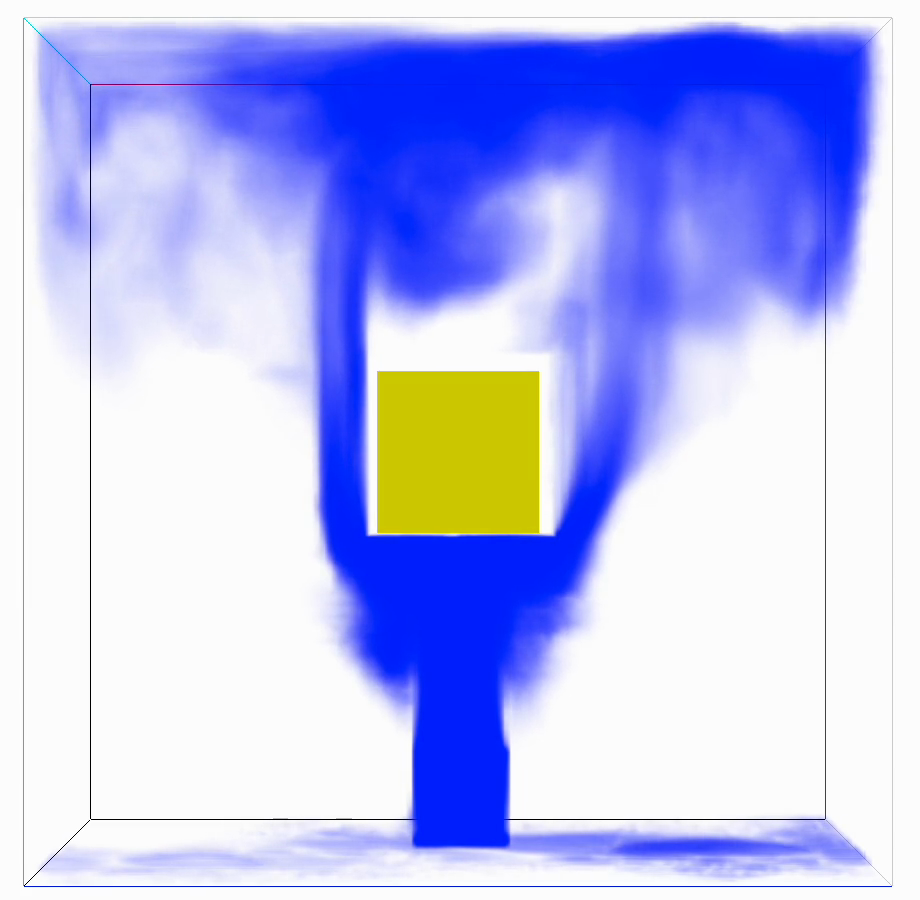
\includegraphics[width=1.0\linewidth]{movies/obstacle_dev1.png}
\caption{既存手法}
   \end{figure}
    \end{column}
    \begin{column}{0.33\textwidth}
       \begin{figure}
\includemovie[autoplay, repeat,poster=movies/obstacle_dev2.png, label=dev2]{40mm}{40mm}{movies/obstacle_dev2_color.mp4}
%		 	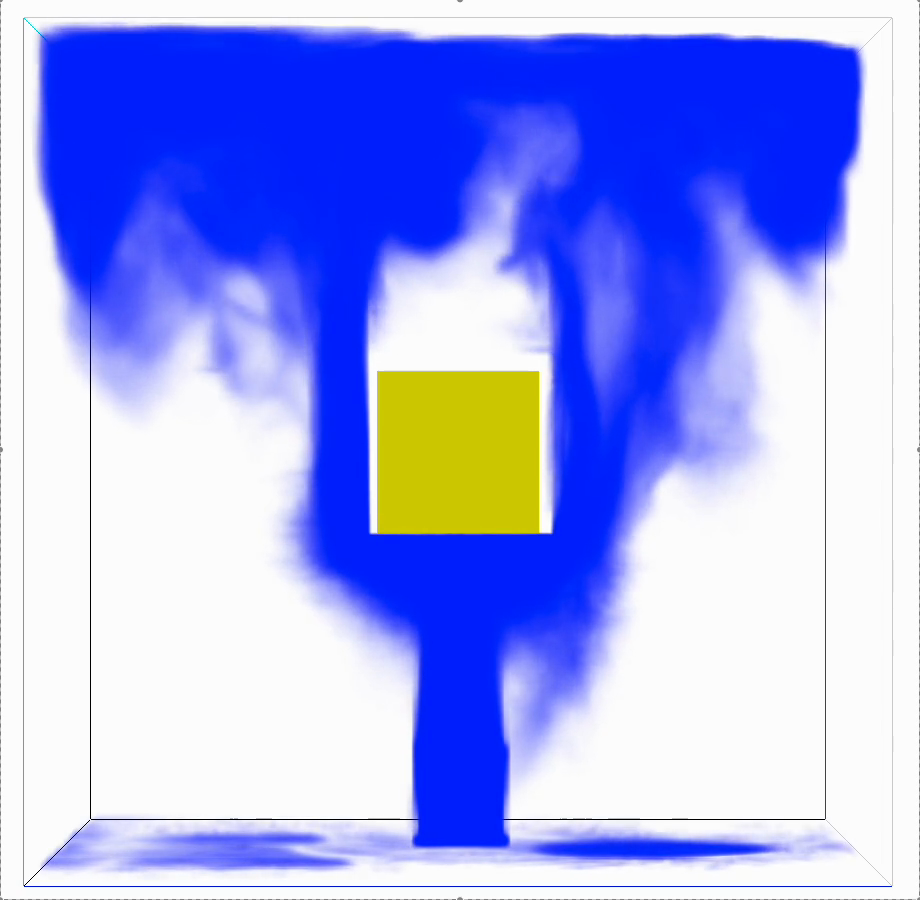
\includegraphics[width=1.0\linewidth]{movies/obstacle_dev2.png}
\caption{提案手法}
   \end{figure}
    \end{column}
\end{columns}
\end{frame}
  %%%%%%%%%%%%%%%%%%%%%%%%%%%%%%%%%%%%%%%%%%%%%%%%%%%%%%%%%%%%%%%%%
  
  %16
 \begin{frame}
 \frametitle{おわりに}
\begin{block}{結論}
\begin{itemize}
	\item スナップショット行列の分割による手法を提案した.
	\item 部分空間の前処理の計算負荷の軽減に成功した.
	\item 流れの様子が急激に変化し,見た目に影響する場合がある.
\end{itemize}
\end{block}
\begin{block}{今後の研究}
\begin{itemize}
	\item 分割の最適化
	\item 分割前後の流速の変化を軽減
	\item 離散コサイン変換を用いた圧縮手法[Jones et al. 2016]への適用
\end{itemize}
\end{block}
\end{frame}
%%%%%%%%%%%%%%%%%%%%%%%%%%%%%%%%%%%%%%%%%%%%%%%%%%%%%%%%%%%%%%%%%%%%%%%%%

%%%%%%%%%%%%%%%%%%%%%%%%%		印刷しない		%%%%%%%%%%%%%%%%%%%%%%%%%%%%%%%%%%
\begin{thebibliography}{99}
\beamertemplatetextbibitems
\bibitem{subspaceDCT}
A. D. Jones, P. Sen, and T. Kim. Compressing fluid subspaces. \textit{Proceedings of the ACM SIGGRAPH/Eurographics Symposium on Computer Animation}, 77--84, 2016.

\bibitem{Chorin}
A. J. Chorin. Numerical solution of the navier-stokes equations. \textit{Mathematics of Computation}, 22(104):745--762, 1968.

\bibitem{projection_base}
A. Treuille, A. Lewis, and Z. Popovi\'{c}. Model reduction for real-time fluids. \textit{ACM Transactions on Graphics}, 25(3):826--834, 2006.

\bibitem{stam}
J. Stam. Stable fluids. In \textit{SIGGRAPH 99 Conference Proceedings, Annual Conference Series}, pages 121--128, 1999.

\bibitem{fedkiw}
R. Fedkiew, J. Stam, and H. Jensen. Visual simulation of smoke. In \textit{Proceedings of SIGGRAPH 01}, 15--22, 2001.

%\bibitem{subspace}
%T. Kim and J. Delaney. Subspace fluid re-simulation. \textit{ACM Transactions on Graphics}, 32(4):62:1--62:9, 2013.

  %%%%%%%%%%%%%%%%%%%%%%%%%%%%%%%%%%%%%%%%%%%%%%%%%%%%%%%%%%%%%%%%%
  
  %質疑
 \begin{frame}
 \frametitle{質疑応答}
\begin{block}{シミュレーションの条件変更}
\begin{itemize}
	\item タイムステップを変更
	\item 障害物を変更
\end{itemize}
\end{block}
\begin{columns}
    \begin{column}{0.33\textwidth}
   \begin{figure}
\includemovie[autoplay, repeat,poster=movies/obstacle_origin.png, label=dt]{40mm}{40mm}{movies/dt.mp4}
%		 	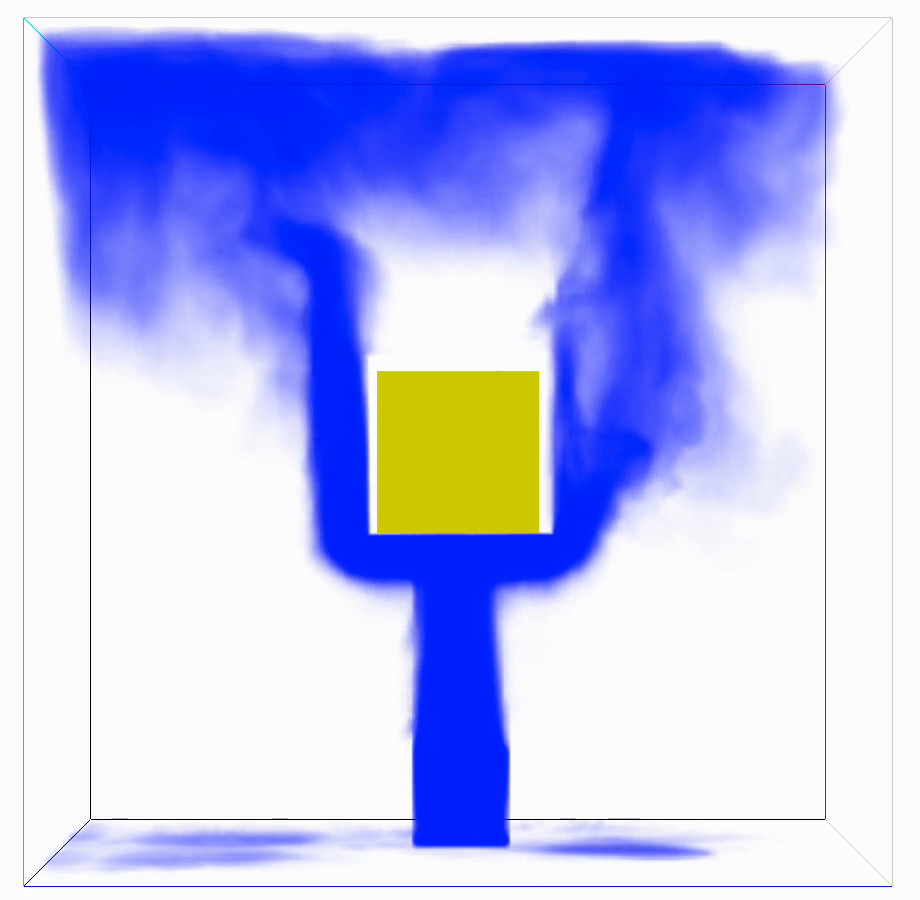
\includegraphics[width=1.0\linewidth]{movies/obstacle_origin.png}
\caption{タイムステップを変更}
   \end{figure}
    \end{column}
    \begin{column}{0.33\textwidth}
       \begin{figure}
\includemovie[autoplay, repeat,poster=movies/obstacle_origin.png, label=dev20]{40mm}{40mm}{movies/obstacle_dev10.mp4}
%		 	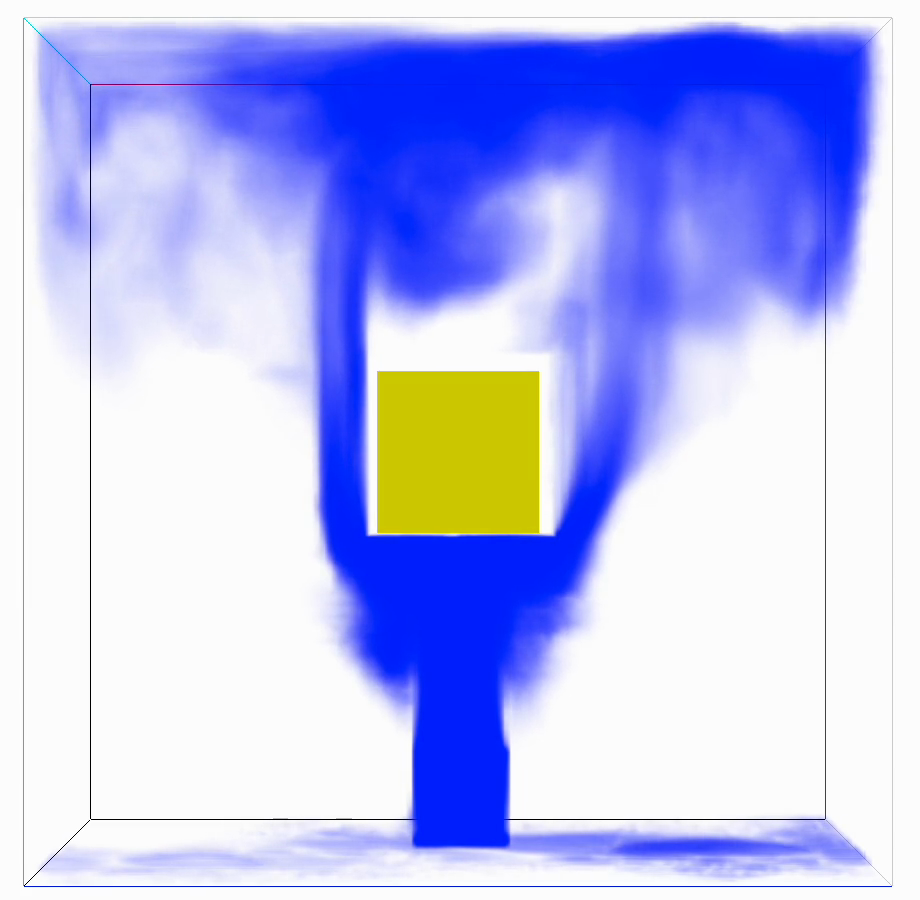
\includegraphics[width=1.0\linewidth]{movies/obstacle_dev1.png}
\caption{大きな分割数}
   \end{figure}
    \end{column}
 \end{columns}

\end{frame}
  %%%%%%%%%%%%%%%%%%%%%%%%%%%%%%%%%%%%%%%%%%%%%%%%%%%%%%%%%%%%%%%%%
  
  %質疑
 \begin{frame}
 \frametitle{質疑応答}
\begin{block}{その他の計算時間}
\begin{itemize}
	\item 圧力項$\bm{p} = \bm{A}^{-1}\bm{b}$は反復回数20回,\text{330ms/f} $\to$ 6\textmu s/f
	\item 粘性項\text{440ms/f} $\to$ 4\textmu s/f
	\item 部分空間から全次元へ射影 1.34ms
\end{itemize}
\end{block}
\end{frame}
%%%%%%%%%%%%%%%%%%%%%%%%%%%%%%%%%%%%%%%%%%%%%%%%%%%%%%%%%%%%%%%%%%%%%%%%%

\end{thebibliography}
\end{document}